\section{Results}
\label{sec:results}

\subsection{Accuracy}
\label{sec:accuracy}
% Numbers: bench/cluster-accuracy-pruned/report.csv and BENCHMARK.md (scikit-learn SOREL split, rpart/J48/YaDT notes).
Before comparing training times, we verify that our implementations match the test accuracy of established libraries. Each tool grows one pruned tree on the full training set at depth limits of 5, 10, 15, and 20 (Table~\ref{tab:accuracy}). All tools use the same fixed pruning rules without tuning. For CART, minimal cost-complexity pruning ($\alpha = 10^{-5}$) is applied natively by rpart and post hoc to the trees of scikit-learn, cuML, and XGBoost. For C4.5, all tools use error-based pruning with a confidence factor of 0.25. All five of our implementations produce the exact same tree in every case.

% bench/cluster-accuracy-pruned/report.csv (one run per case, 2026-11-24/25, ./tree 4de42544, tree code as 7f98876f).
% test_accuracy of each tool, pruned trees only (pruned=True).
\begin{table}[tbp]
\caption{Test accuracy (\%) of a single pruned tree by depth limit. Ours: identical tree across all five implementations. --: no result (rpart exceeds its $2^{31}-1$ value limit; XGBoost runs out of GPU memory; YaDT not run).}
\label{tab:accuracy}
\centering
\footnotesize
\setlength{\tabcolsep}{2.2pt}
\renewcommand{\arraystretch}{0.95}
\begin{tabular}{@{}lr*{5}{c}@{\hspace{6pt}}*{3}{c}@{}}
\toprule
 & & \multicolumn{5}{c@{\hspace{6pt}}}{CART} & \multicolumn{3}{c}{C4.5} \\
\cmidrule(l{2pt}r{6pt}){3-7}\cmidrule(l{2pt}){8-10}
Dataset & Depth & Ours & scikit-learn & rpart & cuML & XGBoost & Ours & J48 & YaDT \\
\midrule
SUSY & 5 & 77.16 & 77.16 & 77.16 & 77.10 & 77.09 & 77.10 & 77.10 & 76.74 \\
 & 10 & 78.99 & 78.99 & 78.99 & 79.08 & 79.05 & 78.64 & 78.64 & 78.76 \\
 & 15 & 79.50 & 79.50 & 79.50 & 79.43 & 79.49 & 79.22 & 79.23 & 79.47 \\
 & 20 & 79.55 & 79.55 & 79.55 & 79.47 & 79.53 & 79.45 & 79.45 & 79.60 \\
\addlinespace[2pt]
HIGGS & 5 & 66.42 & 66.42 & 66.42 & 66.39 & 66.42 & 60.99 & 60.99 & 66.55 \\
 & 10 & 70.47 & 70.47 & 70.46 & 70.45 & 70.47 & 63.73 & 63.75 & 70.10 \\
 & 15 & 71.55 & 71.55 & 71.52 & 71.53 & 71.56 & 67.31 & 67.32 & 71.71 \\
 & 20 & 71.59 & 71.59 & 71.56 & 71.59 & 71.63 & 69.02 & 69.06 & 72.13 \\
\addlinespace[2pt]
MNIST8M & 5 & 62.33 & 62.33 & -- & 61.72 & 62.33 & 45.57 & 45.57 & 45.57 \\
 & 10 & 84.53 & 84.53 & -- & 84.53 & 84.53 & 74.65 & 74.65 & 74.65 \\
 & 15 & 89.94 & 89.94 & -- & 89.97 & -- & 82.02 & 82.02 & 82.02 \\
 & 20 & 90.47 & 90.47 & -- & 90.54 & -- & 87.59 & 87.59 & 87.59 \\
\addlinespace[2pt]
ECBDL'14 15M & 5 & 98.32 & 98.32 & -- & 98.32 & 98.32 & 98.32 & 98.32 & -- \\
 & 10 & 98.32 & 98.32 & -- & 98.32 & 98.32 & 98.32 & 98.32 & -- \\
 & 15 & 98.32 & 98.32 & -- & 98.32 & 98.32 & 98.32 & 98.30 & -- \\
 & 20 & 98.32 & 98.32 & -- & 98.32 & 98.32 & 98.11 & 98.08 & -- \\
\addlinespace[2pt]
SOREL 4M & 5 & 84.49 & 85.08 & -- & 85.15 & 85.00 & 76.25 & 76.25 & -- \\
 & 10 & 92.54 & 92.74 & -- & 92.59 & 92.65 & 78.30 & 78.30 & -- \\
 & 15 & 94.87 & 94.84 & -- & 95.17 & 95.19 & 79.57 & 79.57 & -- \\
 & 20 & 96.12 & 96.10 & -- & 96.09 & 96.26 & 83.17 & 83.17 & -- \\
\bottomrule
\end{tabular}
\end{table}

Across the exact CPU baselines, our CART trees match scikit-learn node for node on four of the five datasets. They also stay within 0.03 percentage points (pp) of rpart where rpart can run. The only exception is scikit-learn on SOREL 4M. Because it ignores splits between values closer than $10^{-7}$, it skips the exact split below the root. Its trees then score up to 0.59\,pp higher at depths 5 and 10 and match ours from depth 15 on. For C4.5, our trees match Weka J48 on MNIST8M and stay within 0.04\,pp on all other datasets. YaDT matches our trees on MNIST8M as well, but uses a different threshold rule on HIGGS, producing a more CART-like tree that scores 3.1--6.4\,pp higher.

Histogram binning has little effect on test accuracy on these datasets. Although cuML and XGBoost split only at bin edges and differ from our predictions on up to 6\,\% of test samples, their accuracy stays within 0.1\,pp of ours on SUSY, HIGGS, and MNIST8M. The one larger gap ($-0.61$\,pp for cuML on MNIST8M at depth 5) lies within the $\pm 1$\,pp sampling margin of the 10,000-sample test set. On SOREL 4M, binned splits generalize slightly better than the greedy exact split, by up to 0.66\,pp. Exact search therefore preserves fidelity to the reference CART and C4.5 algorithms rather than improving accuracy over binning.

Algorithm choice and pruning strength matter far more than the implementation. On HIGGS, MNIST8M, and SOREL 4M, CART outperforms C4.5 by 2.6--16.8\,pp in both our code and J48. The fixed $\alpha = 10^{-5}$ works well on SUSY and HIGGS, shrinking depth-20 trees more than 200-fold with no loss in accuracy. However, it over-prunes MNIST8M and SOREL 4M (losing 2.1 and 0.8\,pp at depth 20) and collapses every CART tree on ECBDL'14 15M (98.32\,\% majority class) to a single leaf. Choosing the right pruning strength thus requires tuning per dataset (Section~\ref{sec:intro}).

\subsection{Training Time}
\label{sec:time}

Table~\ref{tab:time} and Fig.~\ref{fig:bars} summarize the training times of our five implementations at depth 10. Most of the speedup comes from algorithmic optimizations and multicore parallelism, with GPU execution adding a smaller factor on top. On \texttt{epyc}, \ImplSerialOpt{} is 16--35$\times$ faster than \ImplSerialBase{} because it presorts each attribute once and skips provably suboptimal thresholds (Section~\ref{sec:impl-serial}). Adding 48-core parallelism in \ImplParallel{} yields another 14--40$\times$ speedup, with the largest gains on wide datasets. It trains a tree on the full ECBDL'14 and SOREL-20M datasets in 9--16\,s. On the H100, \ImplGpu{} is a further 1.1--1.7$\times$ faster on the real-world datasets and 2.2--2.5$\times$ faster on Chess~$10^9$. On SUSY, about 0.13\,s of fixed GPU setup leaves little room for further speedup. At depth 10, \ImplHybrid{} is slower than \ImplGpu{} on every dataset. Allocating its handoff buffers adds roughly 0.1\,s of setup that shallow trees cannot amortize, making it 2--6\,\% slower on the large real-world datasets and up to 70\,\% slower on SUSY and HIGGS.

% Cells of this work: the final runs, means of bench/cluster-<data>/
% {simple,serial,cpu}-epyc-<data> (epyc; 8fe0c73d/82745fb5 2026-11-17, long
% one-thread runs 81bf6e6c 2026-11-19/20, --simple full ECBDL/SOREL topped up to
% 10 runs 2026-11-21/26) and {gpuonly,cuda}-hopper-<data>
% (7f98876f, job 789, 2026-11-23, GPU setup timed).
% Chess 10^9: bench/cluster-chess/{simple,serial,cpu}-epyc-chess_1b, {gpuonly,cuda}-hopper-chess_1b (10 runs).
\begin{table}[tbp]
\caption{Mean training time (s) for one unpruned tree at depth $\le 10$, including GPU setup. CPU runs use \texttt{epyc}; GPU runs use the H100 (\texttt{hopper}). --: does not fit in 80\,GiB of VRAM. Means of 10 runs per cell.}
\label{tab:time}
\centering
\small
\setlength{\tabcolsep}{2.4pt}
\newcommand{\impl}[1]{\multicolumn{2}{c}{\parbox[b]{17mm}{\centering\hyphenpenalty=10000 #1}}}
\begin{tabular}{@{}l*{10}{r}@{}}
\toprule
 & \impl{\ImplSerialBase} & \impl{\ImplSerialOpt} & \impl{\ImplParallel} & \impl{\ImplGpu} & \impl{\ImplHybrid} \\
\cmidrule(l{2pt}r{2pt}){2-3}\cmidrule(l{2pt}r{2pt}){4-5}\cmidrule(l{2pt}r{2pt}){6-7}\cmidrule(l{2pt}r{2pt}){8-9}\cmidrule(l{2pt}){10-11}
Dataset & CART & C4.5 & CART & C4.5 & CART & C4.5 & CART & C4.5 & CART & C4.5 \\
\midrule
SUSY          & 70.3     & 76.9     & 2.61 & 2.49 & 0.179 & 0.184 & 0.154 & 0.172 & 0.262 & 0.272 \\
HIGGS         & 237      & 259      & 7.89 & 7.42 & 0.348 & 0.366 & 0.221 & 0.243 & 0.329 & 0.349 \\
ECBDL'14      & 5,914    & 6,969    & 316  & 323  & 9.21  & 9.73  & --    & --    & --    & --    \\
\quad 15M     & 2,316    & 2,628    & 148  & 149  & 4.47  & 4.73  & 2.83  & 2.86  & 2.94  & 2.97  \\
MNIST8M       & 1,896    & 1,980    & 115  & 114  & 3.26  & 3.39  & 2.25  & 2.25  & 2.38  & 2.36  \\
SOREL-20M     & 12,527   & 12,903   & 608  & 591  & 15.1  & 15.5  & --    & --    & --    & --    \\
\quad 4M      & 2,939    & 3,127    & 177  & 173  & 5.00  & 5.04  & 2.95  & 3.29  & 3.05  & 3.35  \\
Chess $10^9$  & 922      & 1,039    & 39.0 & 42.2 & 1.63  & 1.98  & 0.741 & 0.792 & 0.841 & 0.893 \\
\bottomrule
\end{tabular}
\end{table}

% bench/cluster-<data>/ as the tables; paper/tools/charts.py bars
\begin{figure}[tbp]
\centering
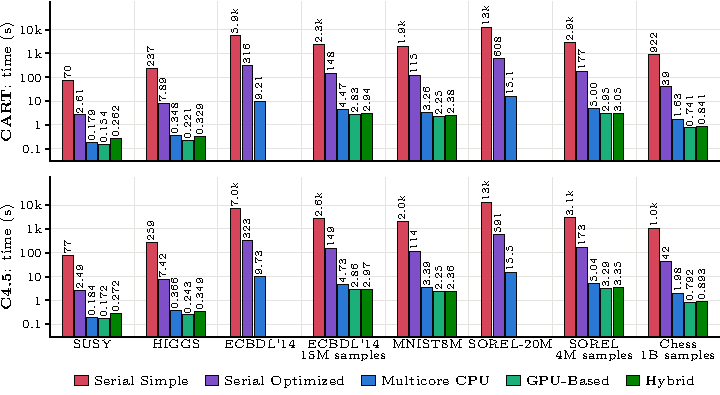
\includegraphics[width=\textwidth]{results-bars.pdf}
\caption{Training time per tree. Missing bars: the dataset does not fit in GPU memory. {\color{red}\textbf{[Candidate for removal]}}}
\label{fig:bars}
\end{figure}

Across servers, memory bandwidth accounts for most of the performance gap on the CPU. Single-threaded \ImplSerialBase{} runs within 16\,\% of the same speed on \texttt{dell} and \texttt{epyc}, whereas 48-thread \ImplParallel{} takes up to 3$\times$ longer on \texttt{dell} on the large datasets because only half of its memory channels are populated. Between the two GPUs, the H100 is 1.4--1.6$\times$ faster than the A100 on the large datasets. On SUSY, the A100 is slightly faster due to shorter fixed setup.

\paragraph{Comparison with existing libraries.}
Figure~\ref{fig:libs} compares training time and peak memory on HIGGS and MNIST8M against established CPU and GPU libraries. On one thread, \ImplSerialOpt{} trains the same CART trees 27$\times$ faster than scikit-learn on HIGGS and 8.8$\times$ faster on MNIST8M, and C4.5 trees 103--147$\times$ faster than Weka J48. On 48 threads, \ImplParallel{} is 2.8$\times$ faster than YaDT on MNIST8M and 49$\times$ faster on HIGGS. On the H100, \ImplGpu{} outperforms the histogram-based GPU libraries cuML (128 bins) and XGBoost (256 bins) by 2.4--3.3$\times$, even though it evaluates every distinct threshold. Presorting does require more memory: on the large datasets, \ImplSerialOpt{} and \ImplParallel{} use about three times the dataset size in RAM, and \ImplGpu{} uses about twice the dataset size in VRAM.

% CPU: bench/cluster-cpu-vs-others/vs-epyc-{higgs,mnist8m} (ours and the libraries in one job);
% GPU CART: cluster-gpu-vs-others/one-tree/vs-hopper-{higgs,mnist8m}; GPU C4.5 and Serial Simple:
% cluster-<data>/{gpuonly,cuda}-hopper-<data>, simple-epyc-<data>. paper/tools/charts.py libs
\begin{figure}[tbp]
\centering
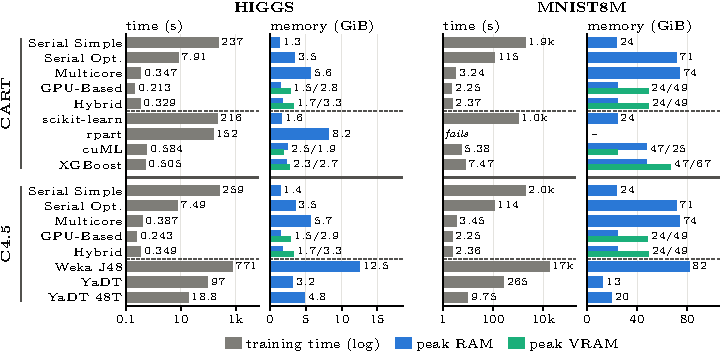
\includegraphics[width=\textwidth]{results-libs.pdf}
\caption{Training time and peak memory compared with existing libraries (depth $\le 10$). GPU memory labels read RAM/VRAM; dashed lines separate ours from external libraries.}
\label{fig:libs}
\end{figure}

Figure~\ref{fig:gpulibs} breaks down the GPU training phases on HIGGS and MNIST8M. Our presort overlaps with the host-to-device upload, whereas cuML and XGBoost prepare inputs or build bins only after the upload finishes (2.35\,s for XGBoost on MNIST8M). Tree construction is also faster (65\,ms vs.\ 253--303\,ms on HIGGS at depth 10). At depth 30, the histogram libraries must build per-node histograms across a much larger tree, widening \ImplGpu{}'s lead to 4.2$\times$ over cuML and 24$\times$ over XGBoost. At this depth, \ImplHybrid{} finishes 1.2$\times$ faster than \ImplGpu{} by offloading small subtrees to the CPU.

% bench/cluster-gpu-vs-others/one-tree/vs-hopper-{higgs,mnist8m,higgs-depth30}/results.jsonl
% (job 789, 2026-11-23, ./tree 7f98876f, 10 runs a tool); paper/tools/charts.py gpulibs
\begin{figure}[tbp]
\centering
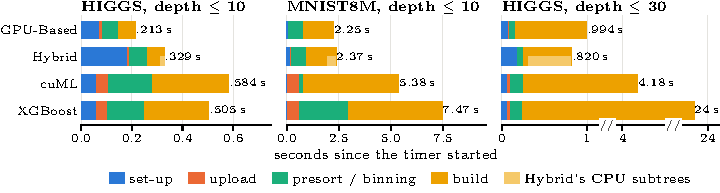
\includegraphics[width=\textwidth]{results-gpulibs.pdf}
\caption{Training phases of one CART tree on the H100. Hatched spans mark concurrent phases; ratios are relative to \ImplGpu{}.}
\label{fig:gpulibs}
\end{figure}

\paragraph{Deep trees.}
To see when hybrid execution pays off, Fig.~\ref{fig:depth}a compares \ImplGpu{} and \ImplHybrid{} across depth limits on three datasets and both GPUs. At depths 5 and 10, \ImplGpu{} wins everywhere (ratios of 0.57--0.98) because few nodes are small enough to hand off. \ImplHybrid{} breaks even around depth 15 on MNIST8M and SOREL 4M (CART), and at depths 20--25 on HIGGS. On SOREL 4M C4.5, it stays within 3\,\% of \ImplGpu{} up to depth 30. Without a depth limit, \ImplHybrid{} is faster in every configuration on both GPUs, reaching up to 1.61$\times$ on MNIST8M (1.52$\times$ for CART on the H100) and up to 1.83$\times$ on HIGGS.

Figure~\ref{fig:depth}b shows the execution breakdown on unrestricted MNIST8M CART. \ImplGpu{} processes every sparse deep level on the GPU, spending 14\,\% of total time on host kernel-launch and synchronization overhead. In \ImplHybrid{}, CPU threads grow handed-off subtrees depth-first while the GPU processes larger nodes. Both devices run concurrently for 61\,\% of the training time, and host overhead drops to 1\,\%. The size of this gain depends on tree shape. Bushy trees such as HIGGS (2.86 million CART nodes without a depth limit) generate many small subtrees for the CPU. In contrast, long, narrow trees such as SOREL 4M (CART depth 231) peel off only a few samples per level from large nodes, keeping most work on the GPU and limiting the speedup to 1.07--1.18$\times$.

% bench/hybrid-vs-gpu-only/{cuda,gpuonly}-{hopper,ampere}-{higgs,mnist8m,sorel_4m} (10 runs a
% case), profile/{cuda,gpuonly}-hopper-mnist8m; paper/tools/charts.py depth_ratio
\begin{figure}[tbp]
\centering
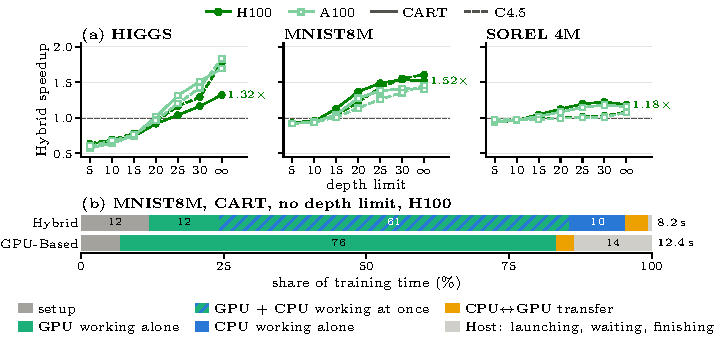
\includegraphics[width=\textwidth]{results-depth.pdf}
\caption{\ImplHybrid{} against \ImplGpu{}: (a)~speedup by depth limit ($>1$: \ImplHybrid{} faster) and (b)~time share by active device.}
\label{fig:depth}
\end{figure}

\subsection{Scaling in Threads and Samples}
\label{sec:scaling}

Figure~\ref{fig:scaling} shows how \ImplParallel{} scales up to 48 threads relative to single-threaded \ImplSerialOpt{}. Scaling improves with the number of attributes: on MNIST8M (784 attributes), \texttt{epyc} scales almost linearly across the first socket and reaches 34.9$\times$ for CART (32.8$\times$ for C4.5) at 48 threads. On HIGGS (28 attributes, 0.35\,s at 48 threads), shorter runtime and fewer attributes limit speedup to 22.8$\times$. On \texttt{dell}, scaling falls behind from 8 threads onward because of its lower memory bandwidth.

% bench/cluster-cpu-scaling/cpu-{epyc,dell}-{higgs,mnist8m}/scaling.csv; paper/tools/charts.py scaling_final
\begin{figure}[tbp]
\centering
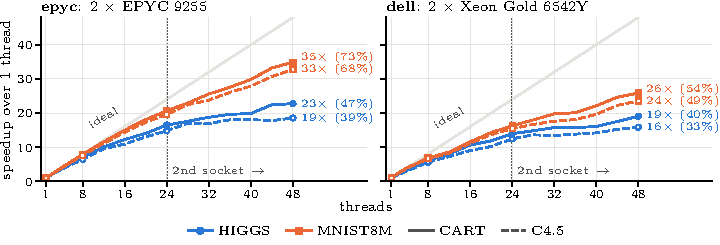
\includegraphics[width=\textwidth]{results-scaling.pdf}
\caption{Speedup of \ImplParallel{} over single-threaded \ImplSerialOpt{}; end labels give speedup and parallel efficiency at 48 threads.}
\label{fig:scaling}
\end{figure}

To isolate sample-count scaling from tree growth, Fig.~\ref{fig:chess} uses the $3 \times 3$ checkerboard, which always produces the same 17-node tree. At $10^7$ samples, fixed GPU setup makes \ImplGpu{} and \ImplHybrid{} slower than \ImplParallel{} on \texttt{epyc} (0.13\,s and 0.23\,s vs.\ 0.05\,s). Between $10^7$ and $10^8$ samples, \ImplGpu{} pulls ahead and reaches a 2.2$\times$ speedup at $2 \cdot 10^9$ samples (1.55\,s vs.\ 3.44\,s), with \ImplHybrid{} close behind (1.61\,s); both fit two billion samples in VRAM. Beyond $10^9$ samples, runtime scales roughly linearly with sample count. On \texttt{epyc}, presorting and partitioning dominate, whereas on the H100, partitioning and host--device transfers take most of the time.

% bench/cluster-profiling/{cpu-epyc,gpuonly-hopper,cuda-hopper}-chess_{10m,100m,1b,2b} (profiled runs, CART);
% paper/tools/charts.py chess
\begin{figure}[tbp]
\centering
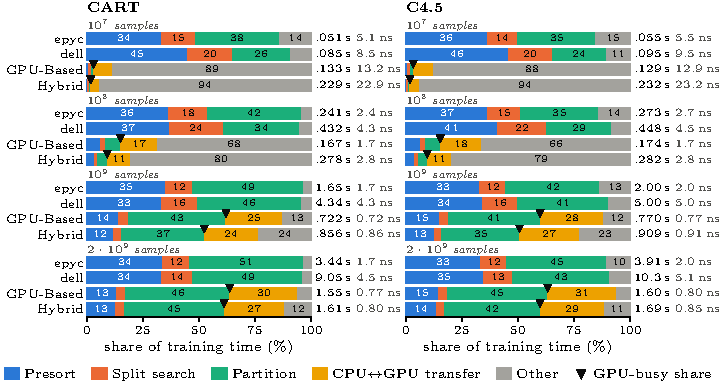
\includegraphics[width=\textwidth]{results-chess.pdf}
\caption{Training time by phase on the $3 \times 3$ checkerboard (CART, profiled runs); totals in seconds above the bars.}
\label{fig:chess}
\end{figure}

\subsection{Energy Consumption}
\label{sec:energy}

Table~\ref{tab:energy} and Fig.~\ref{fig:energy} report whole-server energy per tree. The numbers below refer to C4.5; CART follows the same trends and uses up to 12\,\% less energy on ECBDL'14 15M and up to 18\,\% less on MNIST8M.

Energy consumption is driven primarily by training time. On ECBDL'14 15M at depth 10, mean server power varies only from 264 to 716\,W across implementations, while energy per tree drops 340-fold, from 685 to 2.03\,kJ. \ImplSerialOpt{} cuts energy in proportion to runtime (17$\times$). \ImplParallel{} increases power 2.3$\times$ but still uses 14$\times$ less energy than \ImplSerialOpt{}. \ImplGpu{} on \texttt{hopper} achieves the lowest energy at 2.03\,kJ, or 29\,\% less than \ImplParallel{} on \texttt{epyc}, because it trains 1.7$\times$ faster while drawing only 19\,\% more power. \ImplHybrid{} draws similar power and uses 3\,\% more energy due to its extra setup time.

On unrestricted MNIST8M trees, where all three runs execute on \texttt{hopper}, \ImplHybrid{} also lowers energy. Although keeping the CPUs active alongside the GPU raises mean power by 1.4$\times$ over \ImplGpu{}, \ImplHybrid{} trains 1.58$\times$ faster for C4.5 and reduces energy per tree by 10.5\,\% (and by 4\,\% for CART). Running \ImplParallel{} alone on the same server requires 3.5$\times$ as much energy as \ImplHybrid{}.

% paper/tools/charts.py energy (bench/cluster-power)
\begin{figure}[tbp]
\centering
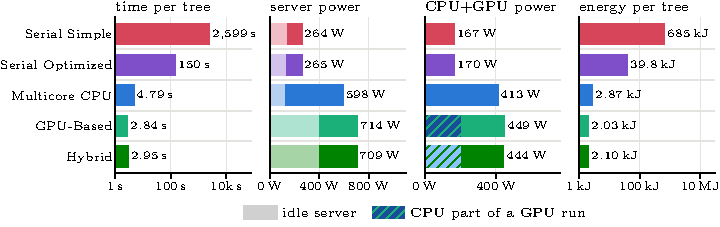
\includegraphics[width=\textwidth]{results-energy.pdf}
\caption{Whole-server time, power, and energy per C4.5 tree at the power supply (idle included). CPU runs in (a) use \texttt{epyc}; all other runs use \texttt{hopper}.}
\label{fig:energy}
\label{fig:energy-deep}
\end{figure}

% bench/cluster-power/ecbdl_15m-depth10/summary.md, final build 81bf6e6c (jobs 559 hopper and
% 528 epyc1, 2026-11-20; Serial trees topped up by jobs 562 hopper and 560 epyc1,
% 2026-11-20/21, and Serial-Simple to 10 by jobs 616 hopper and 657 epyc1, 2026-11-21/22;
% GPU and Hybrid measured again on 7f98876f by job 793, hopper-4, 2026-11-23, the
% old ones listed in hopper/superseded.txt; Hybrid again at its swept --handoff-rows 4096 by
% job 954, hopper-5, 2026-11-25, hopper-4/superseded.txt): whole-server energy at the power supply (meter model),
% training windows only. GPU and hybrid trees after a 2 s CPU warm-up: within 2%
% of the time benchmark's single runs (bench/cluster-power/BENCHMARK.md, Time
% check; warm-up check job 549).
\begin{table}[tbp]
\caption{Mean training time $t$, mean whole-server power $P$ at the power supply (including idle power), and energy $E = P \cdot t$ per tree. {\color{red}\textbf{[Candidate for removal]}}}
\label{tab:energy}
\centering
\small
\setlength{\tabcolsep}{4.5pt}
\begin{tabular}{@{}llrrr@{\hspace{1.4em}}rrr@{}}
\toprule
 & & \multicolumn{3}{c@{\hspace{1.4em}}}{CART} & \multicolumn{3}{c}{C4.5} \\
\cmidrule(r{1.4em}){3-5}\cmidrule{6-8}
 & & $t$ & $P$ & $E$ & $t$ & $P$ & $E$ \\
Implementation & Server & (s) & (W) & (kJ) & (s) & (W) & (kJ) \\
\midrule
\multicolumn{8}{@{}l}{\textit{ECBDL'14 15M, depth $\le$ 10}} \\
\ImplSerialBase & \texttt{epyc}   & 2,298 & 264 & 606  & 2,599 & 264 & 685  \\
\ImplSerialOpt  & \texttt{epyc}   & 147   & 265 & 38.9 & 150   & 265 & 39.8 \\
\ImplParallel   & \texttt{epyc}   & 4.56  & 598 & 2.73 & 4.79  & 598 & 2.87 \\
\ImplGpu        & \texttt{hopper} & 2.80  & 708 & 1.98 & 2.84  & 714 & 2.03 \\
\ImplHybrid     & \texttt{hopper} & 2.92  & 714 & 2.09 & 2.93  & 716 & 2.10 \\
\midrule
\multicolumn{8}{@{}l}{\textit{MNIST8M, no depth limit}} \\
\ImplParallel   & \texttt{hopper} & 28.5  & 915 & 26.1 & 34.3  & 912 & 31.3 \\
\ImplGpu        & \texttt{hopper} & 12.0  & 679 & 8.17 & 15.1  & 661 & 10.0 \\
\ImplHybrid     & \texttt{hopper} & 7.89  & 994 & 7.85 & 9.56  & 937 & 8.95 \\
\bottomrule
\end{tabular}
\end{table}
% MNIST8M block: bench/cluster-power/mnist8m-nodepth/summary.csv (hopper). Hybrid uses the nodepth m
% (8192), confirmed by the 2026-11-24 re-sweep (bench/tools/handoff/RESWEEP-2026-11.md).
